\documentclass{standalone}
\usepackage{ctex}
\usepackage{tikz}
\usetikzlibrary {decorations,arrows.meta,automata,positioning,shadows}
\usetikzlibrary{decorations.pathreplacing,decorations.markings}
\begin{document}
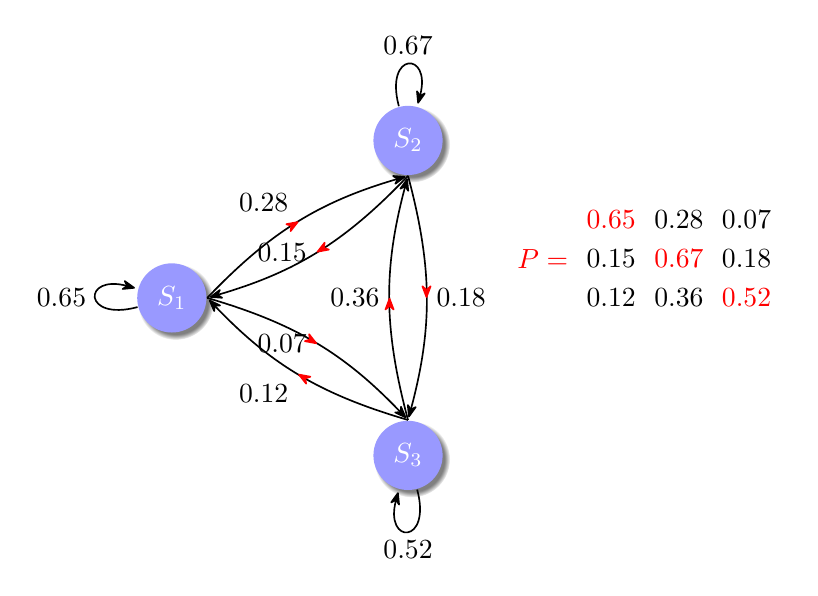
\begin{tikzpicture}[->,>={Stealth[round]},
  shorten >=1pt,auto,node distance=1.8cm,on grid,semithick, %
  every state/.style={fill=blue!40,draw=none,circular drop shadow,text=white},%
  mid arrow/.style={postaction={decorate,decoration={
  markings,mark=at position .5 with {\arrow[red]{Stealth[round]}}}}}]
\node[state] (A)  at (0,0) {$S_1$};
\node[state] (B)  at (3,2) {$S_2$};
\node[state] (C)  at (3,-2) {$S_3$};
\draw[mid arrow] (A.east) to [bend left=15] node{$0.28$} (B.south);
\draw[mid arrow] (A.east) to [bend left=15] node[left] {$0.07$ } (C.north);
\draw[mid arrow] (B.south) to [bend left=15] node[right] {$0.18$} (C.north);
\draw[mid arrow] (B.south) to [bend left=15] node[left] {$0.15$} (A.east);
\draw[mid arrow] (C.north) to [bend left=15] node {$0.12$} (A.east);
\draw[mid arrow] (C.north) to [bend left=15] node {$ 0.36$} (B.south);
\draw (A) edge  [loop left] node {$0.65$} (A);
\draw (B) edge[loop above] node {$0.67$} (B);
\draw (C) edge[loop below] node {$0.52$} (C);
\begin{scope}[xshift=6cm,yshift=0.5cm]
  \matrix[nodes={minimum size=5mm}]{
  &\node[red]{0.65}; &\node{0.28}; &\node{0.07};\\ 
  \node[red]{$P=$};& \node{0.15}; &\node[red]{0.67}; &\node{0.18}; \\
                   & \node{0.12}; &\node{0.36}; &\node[red]{0.52} ;\\ 
    }
    ;
\end{scope}
\end{tikzpicture}
\end{document}
